% Designed Companion Part IV figure
% Intended for \input{...} beside the matching canonical problem.
\begin{figure}[ht]
\centering
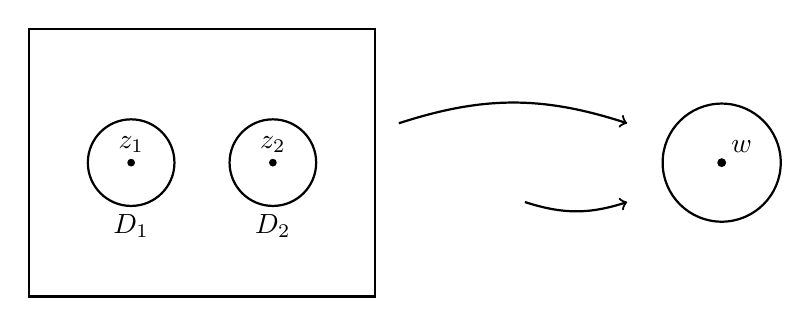
\begin{tikzpicture}[scale=1.0]
  \begin{scope}[xshift=-3.3cm]
    \draw[thick] (-2.2,-1.7) rectangle (2.2,1.7);
    \draw[thick] (-0.9,0) circle (0.55);
    \draw[thick] (0.9,0) circle (0.55);
    \fill (-0.9,0) circle (1.4pt) node[above] {$z_1$};
    \fill (0.9,0) circle (1.4pt) node[above] {$z_2$};
    \node at (-0.9,-0.8) {$D_1$};
    \node at (0.9,-0.8) {$D_2$};
  \end{scope}
  \draw[->,thick] (-0.8,0.5) to[bend left=18] (2.1,0.5);
  \draw[->,thick] (0.8,-0.5) to[bend right=18] (2.1,-0.5);
  \begin{scope}[xshift=3.3cm]
    \draw[thick] (0,0) circle (0.75);
    \fill (0,0) circle (1.6pt) node[above right] {$w$};
  \end{scope}
\end{tikzpicture}
\caption{If a nonconstant limit had $f(z_1)=f(z_2)=w$ with $z_1\ne z_2$, Rouché's theorem on disjoint disks $D_1,D_2$ would force $f_n(z)=w$ to have a solution in each disk for all large $n$, contradicting univalence.}
\label{fig:cp-iv-0037-rouche-two-fibers}
\end{figure}
